\chapter{Parte 5}
\label{cap:p5}

\section{Análise do problema}

Nesta parte do trabalho pretende-se analisar um cenário semelhante à Parte III, em que se pretende reduzir o tempo total do projeto considerando que é possível reduzir a duração de algumas atividades com um custo suplementar. Na Parte III, o custo suplementar de redução era linear. Nesta parte analisa-se a possibilidade de cada atividade poder ter custos não-lineares quando se reduz a sua duração. Para isso, considera-se uma aproximação a uma função não-linear em que se usam duas funções lineares definidas por ramos. Na prática, corresponde a dizer que cada atividade pode estar sujeita a duas reduções de tipos diferentes, em que cada tipo de redução tem um custo associado. Estes dois tipos de redução serão referidos daqui em diante como reduções do tipo 1 e reduções do tipo 2. Como se trata de uma aproximação a uma função não-linear a partir de duas funções, as reduções do tipo 1 deverão ser aplicadas sempre primeiro que as reduções do tipo 2.

\section{Modelo}

\subsection{Parâmetros}

Nesta parte os parâmetros do problema são as precedências das atividades, as suas durações, o custo de ambos os tipos de redução à duração que se pode fazer e os seus respetivos custos suplementares. Em adição, há limites máximos (em unidades de tempo) para cada tipo de redução possível, sendo esses limites também considerados como parâmetros do problema.

Embora os custos normais das atividades sejam um parâmetro do problema, ele não foi considerado na construção do modelo visto o objetivo deste problema ser o de decidir que reduções de tempo se aplicam às atividades, a um custo suplementar mínimo. Os únicos custos relevantes neste contexto são por isso os custos suplementar de redução apenas, não sendo necessário considerar os custos normais de cada atividade na construção do modelo. Os custos normais da atividade foram apenas considerados na análise dos resultados para o cálculo do custo total do projeto (ver secção \ref{p5:resultado}).

\subsection{Variáveis de decisão}
\label{p5:subsec:vardec}

À semelhança das partes anteriores, também aqui se usou o tempo de início de cada atividade como variáveis de decisão, com a mesma nomenclatura apresentada anteriormente. 

Na Parte III introduziram-se variáveis correspondentes às unidades de tempo a reduzir à duração de cada atividade. Nesta parte, cada atividade tem agora associados dois tipos de reduções possíveis. Cada atividade passa agora a ter associadas duas variáveis de decisão, que traduzem as reduções (em unidades de tempo) do tipo 1 e do tipo 2 a aplicar às durações. A nomenclatura das variáveis para as reduções da Parte III teve que ser alterada aqui, para traduzir precisamente o facto de cada atividade poder ter agora dois tipos de redução possíveis, em vez de apenas 1. As novas variáveis apresentam o seguinte formato:

\begin{displaymath}
R_{i\_j}
\end{displaymath}

Onde:
\begin{itemize}
	\item[$i$] Número da atividade
	\item[$j$] Tipo de redução a aplicar (1 ou 2)
\end{itemize}

Assim, $R_{5\_2}$ representa a redução (em unidades de tempo) do tipo 2 a aplicar à duração da atividade 5.


\subsection{Função objetivo}

A função objetivo deste modelo é uma expressão que representa o custo total suplementar de aplicar reduções de tipo 1 e tipo 2 às durações de todas as atividades.

Na Parte III viu-se que saber o custo suplementar de redução para uma atividade correspondia multiplicar o custo de redução/unidade de tempo pelas unidades de tempo de redução que a atividade sofreu. Nesta parte, há dois tipos de reduções, pelo que para uma atividade $i$ o seu custo suplementar de redução total, $C_{i}$, será dado por:

\begin{displaymath}
C_{i} = C_{i\_1} \times R_{i\_1} + C_{i\_2} \times R_{i\_2}
\end{displaymath}

Onde:

\begin{itemize}
	\item[$C_{i\_1}$] Custo por unidade de tempo associada a reduções do tipo 1 na duração da atividade $i$
	\item[$R_{i\_1}$] Unidades de tempo reduzir à duração da atividade $i$ a custo $C_{i\_1}$
	\item[$C_{i\_2}$] Custo por unidade de tempo associada a reduções do tipo 2 na duração da atividade $i$
	\item[$R_{i\_2}$] Unidades de tempo reduzir à duração da atividade $i$ a custo $C_{i\_2}$
\end{itemize}

A função objetivo, $z$, corresponde ao somatório dos custos de redução de todas as atividades, ou seja:

\begin{displaymath}
min~z = \sum C_i
\end{displaymath}

Substituindo os custos das reduções de cada tipo pelo valor dado no enunciado, ficamos com a seguinte função objetivo:

\begin{verbatim}
min: 100 R0_1 + 200 R0_2 + 300 R1_1 + 600 R1_2 + 100 R3_1 + 200 R3_2 + 
400 R4_1 + 800 R4_2 + 800 R5_1 + 1600 R5_2 + 90 R6_1 + 180 R6_2 + 
0 R7_1 + 0 R7_2 + 0 R9_1 + 0 R9_2 + 500 R10_1 + 1000 R10_2 + 300 R11_1 
+ 600 R11_2;
\end{verbatim}


\subsection{Restrições}

Também as restrições serão muito semelhantes às da Parte III.
Em primeiro lugar, mantêm-se as restrições referentes às unidades de tempo máximas que se pode reduzir. Assim cada variável de decisão relativa às reduções a aplicar, terá uma restrição a limitar o seu valor máximo. Visto cada atividade poder estar sujeita a 2 tipos de redução, por cada atividade ter-se-á então 2 restrições relativas aos limites máximos de redução. Em termos genéricos, para a atividade $i$, essas duas restrições podem ser escritas como:

\begin{displaymath}
R_{i\_1} \leq Rmax_{i\_1}; R_{i\_2} \leq Rmax_{i\_2}
\end{displaymath}

Onde:

\begin{itemize}
	\item[$R_{i\_1}$] Variável de decisão --- redução (em unidades de tempo) do tipo 1 a aplicar à atividade $i$
	\item[$R_{i\_2}$] Variável de decisão --- redução (em unidades de tempo) do tipo 2 a aplicar à atividade $i$
	\item[$Rmax_{i\_1}$] Redução máxima de tempo do tipo 1 que é possível aplicar à atividade $i$
	\item[$Rmax_{i\_2}$] Redução máxima de tempo do tipo 2 que é possível aplicar à atividade $i$
\end{itemize}

Por exemplo, para a atividade 5 tem-se as seguintes restrições:

\begin{verbatim}
R5_1 <= 0.5;
R5_2 <= 0.5;
\end{verbatim}

Tal como na Parte III, também as restrições relativas aos tempos de inicio de cada atividade estão presentes neste modelo. Recorde-se que na Parte III tais restrições tinham o seguinte aspecto:

\begin{displaymath}
T_{i} \leq T_{j} + (D_{j} - R{j})
\end{displaymath}

\begin{itemize}
	\item[$T_{i}$] Tempo em que a atividade $i$ inicia
	\item[$T_{j}$] Tempo em que a atividade $j$ inicia
	\item[$D_{j}$] Duração da atividade $j$
	\item[$R_{j}$] Redução de tempo a aplicar na atividade $j$
\end{itemize}

A inequação apresentada em cima parte tem como pressuposto a atividade $j$ preceder a atividade $i$.
A diferença introduzida no modelo desta parte é que cada atividade pode agora ter dois tipos de redução possíveis, pelo que as restrições têm que contar com esse novo fator. Nas restrições da Parte III, o facto de cada atividade poder ver reduzida a sua duração está patente na parcela $(D_{j} - R{j})$ no segundo membro da inequação. Seguindo uma lógica semelhante, dizer que uma atividade pode contar com dois tipos de redução, corresponde a dizer a subtrair uma nova redução à duração. Ou seja:

\begin{displaymath}
T_{i} \leq T_{j} + (D_{j} - R{j\_1} - R{j\_2})
\end{displaymath}

\begin{itemize}
	\item[$R_{j\_1}$] Redução (em unidades de tempo) do tipo 1 a aplicar na atividade $j$
	\item[$R_{j\_2}$] Redução (em unidades de tempo) do tipo 2 a aplicar na atividade $j$
\end{itemize}

Neste modelo era também necessário forçar um tempo de duração total do projeto. Tal como na Parte III, isso foi feito forçando a variável $T_{fim}$ a tomar um valor concreto. Neste modelo usou-se a mesma ideia. Pedia-se que o tempo total do projeto neste modelo fosse inferior em 4 unidades de tempo ao obtido na Parte I. Na Parte I, o tempo total do projeto foi de 26 unidades de tempo. Assim, a restrição que força o tempo total do projeto é:

\begin{verbatim}
Tfim = 26-4;
\end{verbatim}

Visto que os tempos e as reduções não podem ser negativos, neste modelo tem-se ainda restrições de não-negatividade:

\begin{displaymath}
T_{i} \geq 0;  R_{i\_1} \geq 0; R_{i\_2} \geq 0; \forall i_{\in\{ini, 0, 1, 3, 4,5,6,7,9,10,11,fim\}}
\end{displaymath}


\section{Ficheiro \emph{Input}}
\label{p5:sec:fichin}

\begin{verbatim}
/*
=== FUNCAO OBJECTIVO ===
Minimizar os custos suplementares de redução das atividades.
*/
min: 100 R0_1 + 200 R0_2 +
300 R1_1 + 600 R1_2 +
100 R3_1 + 200 R3_2 +
400 R4_1 + 800 R4_2 +
800 R5_1 + 1600 R5_2 +
90 R6_1 + 180 R6_2 +
0 R7_1 + 0 R7_2 +
0 R9_1 + 0 R9_2 +
500 R10_1 + 1000 R10_2 +
300 R11_1 + 600 R11_2;


/*
Reducoes maximas
*/
R0_1 <= 0.5;
R0_2 <= 0.5;

R1_1 <= 1;
R1_2 <= 1;

R3_1 <= 0.5;
R3_2 <= 0.5;

R4_1 <= 1;
R4_2 <= 1;

R5_1 <= 0.5;
R5_2 <= 0.5;

R6_1 <= 1;
R6_2 <= 1;

R7_1 <= 0;
R7_2 <= 0;

R9_1 <= 0;
R9_2 <= 0;

R10_1 <= 0.5;
R10_2 <= 0.5;

R11_1 <= 1;
R11_2 <= 1;


//Nodo Inicial
Tini >= 0 + 0;
//Nodo 0
T0 >= Tini + 0 - Rini;
//Nodo 1
T1 >= T0 + 4 - R0_1 - R0_2;
//Nodo 3
T3 >= T1 + 6 - R1_1 - R1_2;
T3 >= T5 + 4 - R5_1 - R5_2;
T3 >= T4 + 9 - R4_1 - R4_2;
//Nodo 4
T4 >= T0 + 4 - R0_1 - R0_2;
T4 >= T7 + 6 - R7_1 - R7_2;
//Nodo 5
T5 >= T4 + 9 - R4_1 - R4_2;
T5 >= T7 + 6 - R7_1 - R7_2;
T5 >= T10 + 8 - R10_1 - R10_2;
//Nodo 6
T6 >= Tini + 0 - Rini;
//Nodo 7
T7 >= T6 + 5 - R6_1 - R6_2;
//Nodo 9
T9 >= T7 + 6 - R7_1 - R7_2;
T9 >= T11 + 7 - R11_1 - R11_2;
T9 >= T10 + 8 - R10_1 - R10_2;
//Nodo 10
T10 >= T6 + 5 - R6_1 - R6_2;
//Nodo 11
T11 >= T10 + 8 - R10_1 - R10_2;
//Nodo final
Tfim >= T3 + 2 - R3_1 - R3_2;
Tfim >= T5 + 4 - R5_1 - R5_2;
Tfim >= T9 + 2 - R9_1 - R9_2;

/*Forcar reducao de tempo*/
Tfim = 26-4;
\end{verbatim}



\section{\emph{Output} produzido pelo \texttt{lp\_solve}}

\begin{verbatim}
Value of objective function: 820

Actual values of the variables:
R0_1                            0
R0_2                            0
R1_1                            0
R1_2                            0
R3_1                          0.5
R3_2                          0.5
R4_1                            1
R4_2                            0
R5_1                            0
R5_2                            0
R6_1                            1
R6_2                            1
R7_1                            0
R7_2                            0
R9_1                            0
R9_2                            0
R10_1                           0
R10_2                           0
R11_1                           0
R11_2                           0
Tini                            0
T0                              0
Rini                            0
T1                              4
T3                             21
T5                             17
T4                              9
T7                              3
T10                             3
T6                              0
T9                             18
T11                            11
Tfim                           22
\end{verbatim}

\section{Resultado}
\label{p5:resultado}

Os resultados do lpsolve mostram que se consegue reduzir a duração total do projeto em 4 unidades de tempo, passando o projeto a demorar 22 unidades de tempo, com um custo suplementar de 820 unidades monetárias.

O custo total do projeto é dado pela soma dos custos normais das atividades com os custos suplementares de redução às suas durações, sendo este último valor o resultado obtido na função objetivo. O custo normal das atividades é:

\begin{displaymath}
400+1000+300+2000+1000+800+900+300+1600+1400 = 9700~u.m.
\end{displaymath}

O custo total do projeto é dado pela soma dos custos normais das atividades com os custos suplementares de redução às suas durações, sendo este último valor o resultado obtido na função objetivo. Assim, o projeto tem a duração de 22 unidades de tempo, com um custo total de $9700 + 820 = 10520~u.m.$.

O grafo da figura \ref{p5:fig:tempos_inicio} mostra os novos tempos iniciais de cada atividade de acordo com o resultado obtido no lpsolve:

\begin{figure}[<+htpb+>]
	\centering
	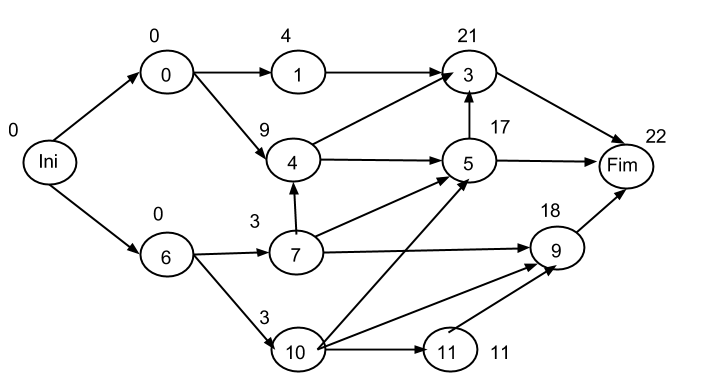
\includegraphics[scale=0.5]{./img/p5_tempos_inicio}
	\caption{Grafo com tempos de inicio das atividades}
	\label{p5:fig:tempos_inicio}
\end{figure}

A figura \ref{p5:fig:reducoes} apresenta o mesmo grafo, com indicação das reduções feitas às atividades e respetivas durações. Os números a roxo indicam as reduções de tipo 1 e os números a verde as reduções de tipo 2.

\begin{figure}[<+htpb+>]
	\centering
	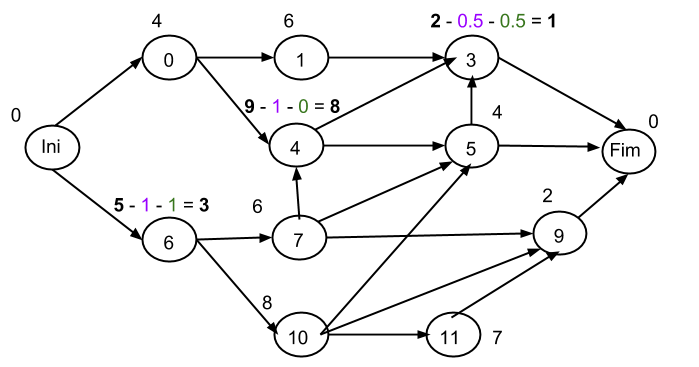
\includegraphics[scale=0.5]{./img/p5_reducoes}
	\caption{Grafo com reduções de tempo às atividades}
	\label{p5:fig:reducoes}
\end{figure}

O Diagrama de Gantt correspondente à execução do projeto encontra-se na figura \ref{p5:fig:diagrama_gantt}:

\begin{figure}[<+htpb+>]
	\centering
	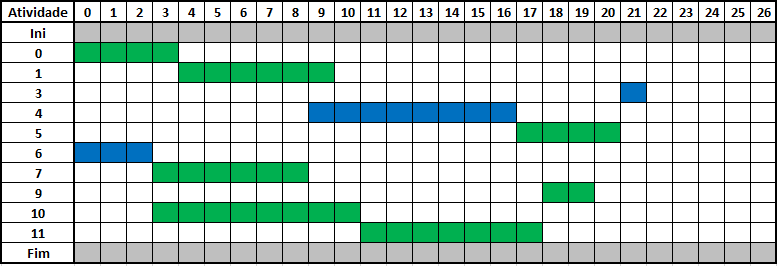
\includegraphics[scale=0.5]{./img/p5_diagrama_gantt}
	\caption{Grafo com reduções de tempo às atividades}
	\label{p5:fig:diagrama_gantt}
\end{figure}

As atividades que sofreram redução encontram-se marcadas a azul.

É interessante também notar que a duração total do projeto é de 22 unidades de tempo, no entanto, se somarmos as novas durações das atividades que na Parte I faziam parte do caminho crítico tem-se uma duração de $3+6+8+1=18$ unidades de tempo. Visto que a duração do projeto não é a mesma do caminho crítico da Parte I, podemos concluir que o caminho crítico se alterou com as reduções aplicadas.

\section{Validação do Modelo}

Para validar os resultados, tanto na função objetivo como nas restrições,
substituímos os valores das variáveis de decisão pelo valor que estas tomam na
solução que o lp\_solve indica como ótima. A ideia é verificar que os valores das
variáveis de decisão obtidos confirmam o valor da função objetivo obedecendo
a todas as restrições.

Para evitar ao máximo o erro humano, a substituição de variáveis foi feita
recorrendo a ferramentas que auxiliaram a substituição automática das variáveis
pelo seu valor.

\subsection{Variáveis de Decisão}

No resultado obtido, todas as variáveis tomam um valor maior ou igual a 0, tal
como seria de esperar.

\subsection{Função objetivo}

Depois da substituição das variáveis pelo seu valor, a função objetivo
fica:\\

$100*0+200*0+300*0+600*0+100*0.5+200*0.5+400*1+800*0+800*0+
1600*0+90*1+180*1+0*0+0*0+0*0+0*0+500*0+1000*0+300*0+600*0$\\

Inserindo a expressão numa calculadora verifica-se que a expressão é igual a 820,
o que confirma o resultado obtido com o \textit{lp\_solve}.

\subsection{Restrições}

\begin{verbatim}

/*
Reducoes maximas
*/
R0_1 <= 0.5;
R0_2 <= 0.5;

0 <= 0.5;
0 <= 0.5;


R1_1 <= 1;
R1_2 <= 1;

0 <= 1;
0 <= 1;

R3_1 <= 0.5;
R3_2 <= 0.5;

0.5 <= 0.5;
0.5 <= 0.5;

R4_1 <= 1;
R4_2 <= 1;

1 <= 1;
0 <= 1;

R5_1 <= 0.5;
R5_2 <= 0.5;

0 <= 0.5;
0 <= 0.5;

R6_1 <= 1;
R6_2 <= 1;

1 <= 1;
1 <= 1;


R7_1 <= 0;
R7_2 <= 0;

0 <= 0;
0 <= 0;

R9_1 <= 0;
R9_2 <= 0;

0 <= 0;
0 <= 0;


R10_1 <= 0.5;
R10_2 <= 0.5;

0 <= 0.5;
0 <= 0.5;


R11_1 <= 1;
R11_2 <= 1;

0 <= 1;
0 <= 1;



//Nodo Inicial
Tini >= 0 + 0;
0 >= 0 + 0;
//Nodo 0
T0 >= Tini + 0 - Rini;
0 >= 0 + 0 - 0;
//Nodo 1
T1 >= T0 + 4 - R0_1 - R0_2;
4 >= 0 + 4 - 0 - 0;
//Nodo 3
T3 >= T1 + 6 - R1_1 - R1_2;
T3 >= T5 + 4 - R5_1 - R5_2;
T3 >= T4 + 9 - R4_1 - R4_2;

21 >= 4 + 6 - 0 - 0;
21 >= 17 + 4 - 0 - 0;
21 >= 9 + 9 - 1 - 0;
//Nodo 4
T4 >= T0 + 4 - R0_1 - R0_2;
T4 >= T7 + 6 - R7_1 - R7_2;
9 >= 0 + 4 - 0 - 0;
9 >= 3 + 6 - 0 - 0;
//Nodo 5
T5 >= T4 + 9 - R4_1 - R4_2;
T5 >= T7 + 6 - R7_1 - R7_2;
T5 >= T10 + 8 - R10_1 - R10_2;
17 >= 9 + 9 - 1 - 0;
17 >= 3 + 6 - 0 - 0;
17 >= 3 + 8 - 0 - 0;
//Nodo 6
T6 >= Tini + 0 - Rini;
0 >= 0 + 0 - 0;
//Nodo 7
T7 >= T6 + 5 - R6_1 - R6_2;
3 >= 0 + 5 - 1 - 1;
//Nodo 9
T9 >= T7 + 6 - R7_1 - R7_2;
T9 >= T11 + 7 - R11_1 - R11_2;
T9 >= T10 + 8 - R10_1 - R10_2;
18 >= 3 + 6 - 0 - 0;
18 >= 11 + 7 - 0 - 0;
18 >= 3 + 8 - 0 - 0;
//Nodo 10
T10 >= T6 + 5 - R6_1 - R6_2;
3 >= 0 + 5 - 1 - 1;
//Nodo 11
T11 >= T10 + 8 - R10_1 - R10_2;
11 >= 3 + 8 - 0 - 0;
//Nodo final
Tfim >= T3 + 2 - R3_1 - R3_2;
Tfim >= T5 + 4 - R5_1 - R5_2;
Tfim >= T9 + 2 - R9_1 - R9_2;
22 >= 21 + 2 - 0.5 - 0.5;
22 >= 17 + 4 - 0 - 0;
22 >= 18 + 2 - 0 - 0;

/*Forcar reducao de tempo*/
Tfim = 26-4;
22 = 26-4;

\end{verbatim}

Assim conclui-se que todas as restrições são respeitadas.










